\section{Kết quả}
\subsection{Bài 1}
Sử dụng kỹ thuật xử lý bit viết chương trình thực hiện các yêu cầu sau:

- Nhập vào số nguyên X (4 byte) có dấu hãy "đọc" dãy bit nhị phân của X và xuất ra màn hình.

- Cho mảng 1 chiều A gồm 32 phần tử là các số 0 hoặc 1. Hãy xây dựng số nguyên X 4 byte có các bit giống với các phần tử mảng A, sau đó xuất X ra màn hình.
	
\begin{figure}[H]
	\centering
	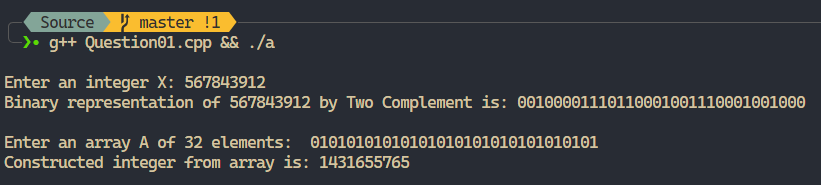
\includegraphics[width=\textwidth]{images/img1.PNG}
	\caption{Chụp màn hình kết quả bài 1.}
\end{figure}

\subsection{Bài 2}

Viết chương trình Nhập vào 2 dãy bit 8 bit (ở dạng bù 2):
Hãy thực hiện các phép tính cộng, trừ, nhân, chia trên 2 dãy bit đã nhập (Lưu ý: thực hiện theo thuật toán đã học).

\begin{figure}[H]
	\centering
	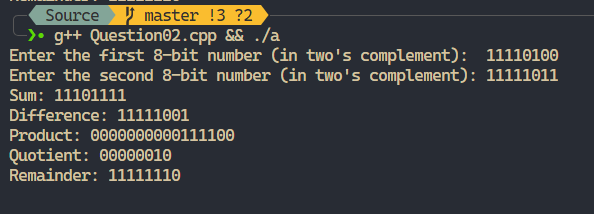
\includegraphics[width=\textwidth]{images/img2.PNG}
	\caption{Chụp màn hình kết quả bài 2.}
\end{figure}
